\chapter{Machine Learning}
% \begin{center}
% \begin{tcolorbox}[enhanced,width=6in,center upper,
%     fontupper=\large,drop fuzzy shadow southwest,
%     colframe=blue!50!black,colback=blue!10]
% Für dieses Unterkapitel ist ein Jupyter-Notebook verfügbar. Siehe \gitresource{Machine Learning.ipynb}  
% \end{tcolorbox}
% \end{center}

\section{Grundzüge von Machine Learning}
Das Ziel von Machine Learning (ML) ist die Reproduktion von biologischem Lernverhalten in Computern. 
Ein Beispiel aus der Objekt-Klassifizierung: Menschen können schnell eine Lampe von einem Buch unterscheiden, obwohl es sehr viele verschiedene Lampen und Bücher gibt. 
Es ist allerdings schwierig, eine formelle Definition von \textit{Lampe} zu geben und somit Algorithmen zu entwerfen. 
Wir Menschen treffen solche Entscheidungen nicht mithilfe von solchen Definitionen, sondern wir benutzen unsere vorherigen Erfahrungen. Eine Lampe ist eine Lampe, weil es unsere vorherigen Erfahrungen mit Lampen widerspiegelt.\\

Da Computer keine Erfahrungen sammeln wie Menschen, brauchen wir eine Methode, um Computern etwas beizubringen. 
Wir müssen folgendes für den Computer bereitstellen:
\begin{enumerate}
    \item \textbf{Datensatz: } z.B. Bilder von Lampen
    \item \textbf{Modell: } in der Biologie ist dies das Gehirn
    \item \textbf{Verlustfunktion: } ein Mass dafür wie falsch die Aussagen sind.
\end{enumerate}
Wenn wir diese haben, können wir den Computer trainieren und dann validieren. 

\subsection{Datensatz}
Ein Datensatz ist eine Tabelle mit beliebig vielen Merkmalen und einem Klassifizierungslabel (\textit{class label}). Die Merkmale können Antworten zu ja-nein-Fragen oder aber auch Zahlen sein. Die Merkmale für eine Lampe können zum Beispiel die folgenden sein:
\begin{itemize}
    \item Ist es hell?
    \item Kann man es aus- und einschalten?
    \item Verwendet es Elektrizität?
\end{itemize}
Das class label ist dann: Ist es eine Lampe?
Wir werden ein Modell so trainieren, dass es aus den Merkmale das class label vorhersagen kann. 

\subsection{Modell}
Ein Modell ist eine Menge von möglichen Algorithmen, die die Merkmale als Argument nehmen 
und ein class label als Antwort zurückgeben. Wir beschriften diese Menge oft 
mit $\mathcal{H}$. $\mathcal{H}$ wird auch als Hypothesenraum bezeichnet. 
Beispiele sind Entscheidungsbäume oder Neuronale Netze bestimmter Struktur. 

\subsection{Verlustfunktion}
Eine Verlustfunktion $L(D,f)$ ist eine Funktion, die einen Datensatz D und eine $f \in \mathcal{H}$ als Argument nimmt und die Fehlerrate der $f$ in $D$ quantifiziert. 
Für Entscheidungsbäume wäre der Anteil von falschen Klassifizierungen eine mögliche Verlustfunktion. Es gibt keine allgemeine Verlustfunktion, sondern man muss eine für das Modell $\mathcal{H}$ auswählen.

\subsection{Training}
Das Training minimiert die Verlustfunktion anhand von Trainingsdaten. Wie man dies spezifisch schafft, ist abhängig von dem Modell und der Verlustfunktion. Es ist oft in Python Packages für verschiedene Modelle implementiert.

\subsection{Validierung}
Für Validierung verwenden wir einen anderen Datensatz $D'$ (also nicht den Trainingsdatensatz und überprüfen, 
dass die von Training ausgewählte $f^* \in \mathcal{H}$ auch für andere Datensätze funktioniert. 
Es kann sein, dass unser Modell nur den Datensatz D auswendig gelernt hat und keine Aussagen über andere Datensätze machen kann. 
Wie müssen deshalb sicherstellen, dass dies nicht der Fall ist.


\section{Ausgewählte Modelle}

Im folgenden werden wir uns einige Machine learning Modelle anschauen. Das Ziel dieses Abschnitts ist, 
Ihnen einerseits einige grundlegende Ideen des maschinellen Lernens zu vermitteln, aber Ihnen anderseits auch 
die Verknüpfung zu den mathematischen Methoden aufzuzeigen, die Sie in der Vorlesung kennengelernt haben.

\subsection{Lineare Regression als Machine Learning Modell}

Wir beginnen mit einem der einfachsten Modelle, der linearen Regression, welche Sie ja bereits in in Kapitel \ref{subsubsec:vl8}
kennengelernt haben. Lineare regression ist eine klassische Methode aus der Statistik. In der Statistik liegt der Fokus auf dem Verstehen, wie eine oder mehrere Variablen eine von diesen Variablen abhängige Grösse erklären. Im maschinellen lernen hingegen sind wir besonders an den Vorhersagen interessiert, die wir durch ein auf die Daten angepasstes Modell erhalten können. 
Darüberhinaus eignen sich lineare Regressionsmodelle, und die darauf aufbauenden linearen Basisfunktionsmodelle, ausgezeichnet, die Grundkonzepte des maschinellen Lernens zu illustrieren. 

Gegeben ist ein Datensatz aus Eingabe/Ausgabepaaren 
\[
    D = \left\{ (x_1,y_1),...,(x_n,y_n) \right\} \subset \mathbb{R} \times \mathbb{R}
\]
und ein Modell der Form:
\[
    f(x, a, b) = ax + b.
\]
Der Hypothesenraum ist also der Raum der linearen Funktionen 
\[
\mathcal{H} = \{a x + b \,| \,a, b \in \mathbb{R}\}.    
\]

Der Fehler, den wir durch eine Vorhersage $\hat{y} =f(x, a, b)$ machen, können wir durch das 
Quadrat des Unterschieds zwischen der Vorhersage und dem tatsächlichen Wert $y$ quantifizieren.
Die Verlustfunktion wird entsprechend wie folgt definiert:
\[
    L(y, \hat{y}) = L(y, f(x, a,b))=  (f(x, a, b) - y)^2.
\]

Um die optimalen Parameter zu finden, minimieren wir die Verlustfunktion über alle Datenpaare $D=\{(x_1, y_1), \ldots, (x_n, y_n)\}$:
\[
    \min_{a, b} \sum_{i=1}^n L(y_i, f(x_i, a, b)).
\]
Da die Verlustfunktion eine quadratische Funktion und das
Modell linear in den Parametern $a$ und $b$ ist, können wir 
die optimalen Parameter durch das Lösen der Normalgleichung (Gleichung~\ref{eq:vl8-28-2}) bestimmen.

\subsection{Lineare Basisfunktionsmodelle}

Der Zusammenhang zwischen den Merkmalen und der Vorhersage ist oft nicht linear.
Ein einfacher, jedoch sehr flexibler Ansatz, um diese einfache linearen Regressionsmodelle zu erweitern, ist die Verwendung von Basisfunktionen. Auch dieses Modell kennen Sie bereits aus Kapitel~\ref{subsubsec:vl8}, in welchem Sie als Basisfunktionen Polynome $m$-ter Ordnung verwendet haben. Neben Polynomen werden im Maschinellen lernen jedoch noch viele weitere 
Funktionen als Basisfunktionen verwendet. 
Ein lineares Basisfunktionsmodell hat die Form:
\[
    f(x, \textbf{w}) = w_0 + \sum_{i=1}^m w_i \phi_i(x),
\]
wobei $\phi_i(x), \, i = 1, \ldots, m$ die Basisfunktionen sind und der 
Vektor $\textbf{w}=(w_1, \ldots, w_m)$ die dazugehörigen Parameter zusammenfasst. 
Da das Modell noch immer linear in den Modellparametern ist, lassen sich die Parameter wieder durch das Lösen der Normalgleichungen bestimmen. Jedoch führt die Transformation mit den Basisfunktionen dazu, dass die durch das Modell $f(x, \textbf{w})$ gemachten Vorhersagen nicht mehr nur lineare Kombinationen der Merkmale sind. 

Eine Interpretation dieser Modelle ist, dass wir eine Eingabe $x$ zuerst durch das Anwenden der Basisfunktionen $\phi_1(x), \ldots, \phi_m(x)$ transformieren, und dann in diesem $m$-Dimensionalem Raum eine lineare Regression durchführen. Die Basisfunktionen sollen also die Daten so transformieren, dass nach der Transformation ein 
einfacher linearer Zusammenhang zwischen den Merkmalen $x_i$ und den Vorhersagen $y_i$ besteht. 
Dies wird in Abbildung~\ref{fig:ml-poly-regression-simple} illustriert. Die Daten wurden dabei anhand der Funktion $f(x) = 3 x^2 + s + 1$ generiert. Als Basisfunktionen werden $\phi_0(x)=x^0, \phi_1(x) = x, \phi_2(x)=x^2$ verwendet. Die Vorhersage entspricht dann genau der gewichteten Summe dieser drei Basisfunktionen mit den Gewichten $w_0 = 1, w_1=1, w_2 = 3$.

\begin{figure}[tb]
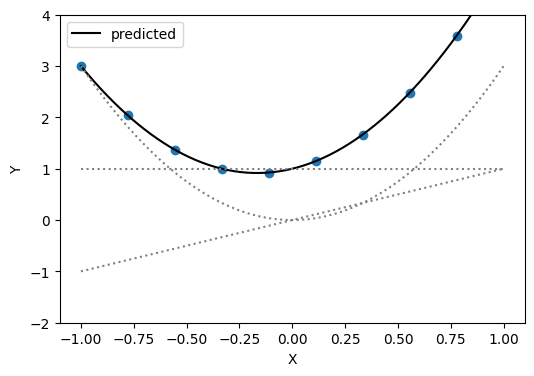
\includegraphics{Figures/ML-poly-regession-simple.png}
\caption{Lineares Basisfunktionenmodell: Die Daten (blaue Punkte) wurden anhand der Funktion $f(x) = 3 x^2 + s + 1$
generiert. Die grauen Linien zeigen die (gewichteten) Basisfunktionen $\phi_0(x)=x^0, \phi_1(x) = x, \phi_2(x)=x^2$. Die Vorhersage (schwarze Linie) entspricht genau der Summe dieser Basisfunktionen.}
\label{fig:ml-poly-regression-simple}
\end{figure}

Abbildung \ref{fig:ml-basisfunktionen-okfit} illustriert eine etwas komplexere Situation. Die Daten (blaue Punkte) wurden anhand einer Sinusfunktion generiert, welche in Rot eingezeichnet ist, und 
dann mit einem Rauschen versehen. Für die Vorhersage wurden Polynomiale Basisfunktionen bis Grad 8 verwendet. 
Die Vorhersagen stimmen gut mit der in rot eingezeichnete wahren Funktion überein. 
Einen noch präziseren Fit an die Daten erhalten wir, wenn wir die Anzahl der Basisfunktionen erhöhen, also zum Beispiel 
Polynome bis Grad 30 als Basisfunktionen nehmen. Das Resultat ist in Abbildung \ref{fig:ml-basisfunktionen-overfitted} gezeigt. Die Daten werden nun perfekt gefittet, aber die
Lösung entspricht nicht dem, was wir  erwarten würden. 
% \begin{figure}[tb]
%     \includegraphics*[width=0.5\textwidth]{Figures/ML-poly-regession-overfitted.png}
%     \label{fig:ml-basisfunktionen-overfitted}
%     \caption{Ein lineares Basisfunktionsmodell mit Polynomialbasisfunktionen bis Grad 20. Die grauen, 
%     gestrichelten Linien zeigen die Basisfunktionen. Die rote Linie zeigt die 
%     wahre Funktion, mit der die Daten generiert wurden. Die schwarze Linie zeigt die 
%     Vorhersage des Modells.}
% \end{figure}


\begin{figure}[tb]
    \begin{subfigure}[b]{0.5\textwidth}
        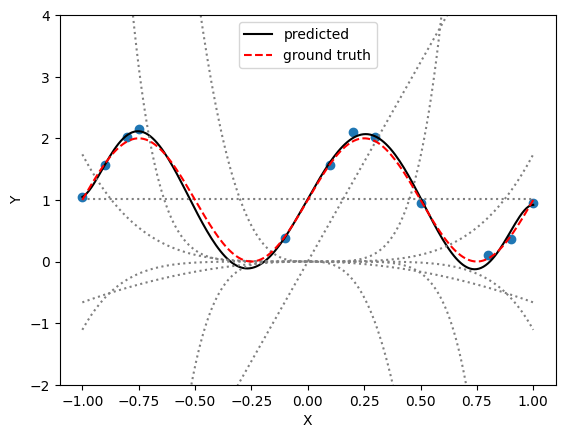
\includegraphics[width=\textwidth]{Figures/ML-poly-regession.png}
        \caption{}
        \label{fig:ml-basisfunktionen-okfit}
    \end{subfigure}
    \hfill
    \begin{subfigure}[b]{0.5\textwidth}
        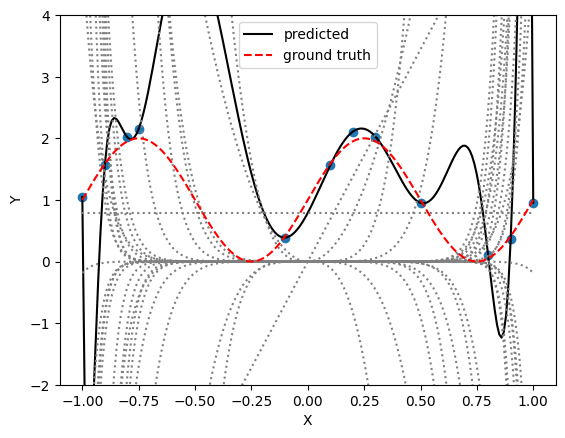
\includegraphics[width=\textwidth]{Figures/ML-poly-regession-overfitted.png}
        \caption{}
        \label{fig:ml-basisfunktionen-overfitted}
    \end{subfigure}
    \caption{Zwei Beispiele für lineare Basisfunktionsmodelle mit Polynomialbasisfunktionen. \subref{fig:ml-basisfunktionen-okfit} zeigt ein Modell mit Polynomen bis Grad 8 und \subref{fig:ml-basisfunktionen-overfitted} ein Modell mit Polynomen bis Grad 30. 
    Die blauen Punkte zeigen die Daten, die rote Linie die wahre Funktion und die Schwarze Linie die Vorhersage des Models.}
    \label{fig:ml-basisfunktionen}
\end{figure}

Dieses Beispiel zeigt mehrere grosse Probleme von polynomialen Basisfunktionsmodellen auf:
Die Basisfunktionen sind global definiert, was bedeutet, dass sie über den gesamten
Definitionsbereich definiert sind. Dies führt dazu, dass die Basisfunktionen in Bereichen,
in denen keine Daten vorhanden sind, zu starken Ausschlägen führen können.
Zudem haben die Basisfunktionen keinerlei Bezug zu den Daten.
Ein weiteres Problem ist, dass die Anzahl der Basisfunktionen manuell festgelegt werden muss 
und nicht von den Daten bestimmt wird. Dies führt dazu, dass das Modell entweder zu
einfach oder zu komplex sein kann.

Wir können einen Teil dieser Probleme lösen, indem wir die Basisfunktionen lokal definieren 
und deren Position automatisch aus den Daten bestimmen. Eine verbreitete, lokale Basisfunktion 
ist die \emph{Radiale Basisfunktion} (RBF), die wie folgt definiert ist:
\[
    \phi_i(x) = \exp\left( -\frac{1}{2} \frac{(x - \mu_i)^2}{s^2} \right).
\]
Die Funktion entspricht von der Form her der unnormalisierten Dichtefunktion der Normalverteilung. 
Der Parameter $\mu_i$ bestimmt die Position der Basisfunktion und $s$ definiert deren Breite. Beachten Sie, dass der Wert von $\phi_i$ gegen 0 geht, wenn die Distanz von Punkt $x$ zu $\mu_i$ gross wird. Wenn wir nun $\mu_i$ so wählen, dass es die Position eines Datenpunktes ist, dann wird die Basisfunktion nur in der Nähe von diesem Datenpunkt gross sein und hat keinen 
Einfluss weit weg von den Datenpunkten. Das Modell besagt also, dass die Vorhersage eines 
neuen Punkts hauptsächlich lokal, von den observierten Werten der Punkte in der Nähe bestimmt wird. Wie gross der Einfluss ist, wird durch den Parameter $s$ bestimmt.
Da die 
Anzahl Basisfunktionen durch die Anzahl Datenpunkte bestimmt ist, wird auch  
die Komplexität des Modells automatisch höher, wenn mehr Daten zum Lernen zur Verfügung stehen. 
Abbildung \ref{fig:ml-rbf} zeigt ein Beispiel für ein lineares Basisfunktionsmodell mit RBFs.
Wir sehen, dass die Vorhersage deutlich besser ist, als für Polynome hohen Grads. 

\begin{figure}[tb]
    \center
    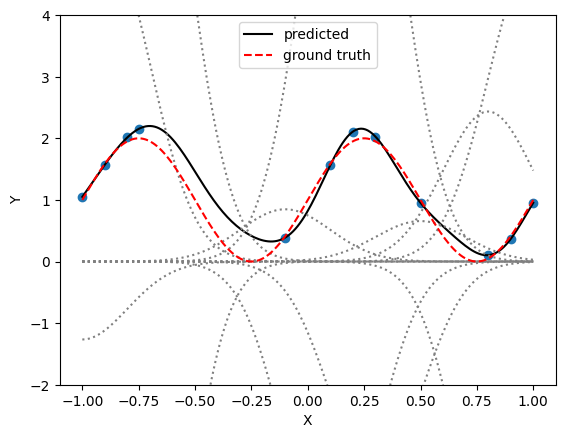
\includegraphics[width=0.5\textwidth]{Figures/ML-rbf-regession.png}
    \caption{Ein lineares Basisfunktionsmodell mit Radialbasisfunktionen. Die grauen, 
    gestrichelten Linien zeigen die Basisfunktionen. Die rote Linie zeigt die 
    wahre Funktion, mit der die Daten generiert wurden. Die schwarze Linie zeigt die 
    Vorhersage des Modells.}
    \label{fig:ml-rbf}        
\end{figure} 


\subsection{Einschub: Regularisierung und Bayesianische Regression}

Mit genügend Basisfunktionen können wir grundsätzlich alle Eingabedaten perfekt durch unser Modell interpolieren. 
Unser Ziel ist aber natürlich nicht, die Eingabedaten perfekt wiederzugeben, sondern das 
zugrundeliegende Muster zu finden, so dass wir gute Vorhersagen machen können. Wie in Abbildung~\ref{fig:ml-basisfunktionen} gezeigt können unterschiedliche Modelle die Daten ganz unterschiedlich erklären. 
% \begin{figure}[tb]
%     \center    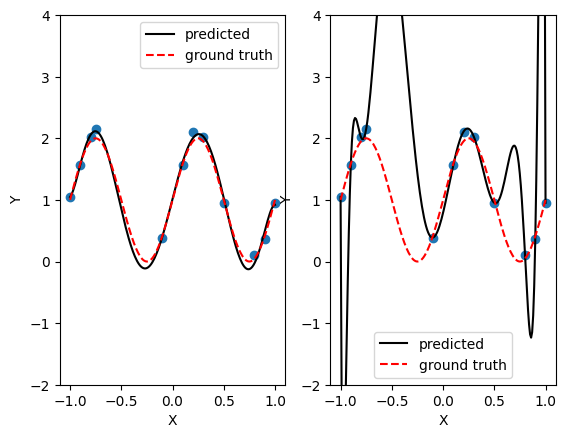
\includegraphics[width=0.7\textwidth]{Figures/ML-overfitting.png}
%     \caption{Zwei mögliche Erklärungen für die gleichen Daten mit verschiedenen Modellen.}
%     \label{fig:ml-overfitting}    
% \end{figure}
Intuitiv bevorzugen wird die Erklärung links, da diese \emph{einfacher} ist. Das Modell wurde so beschränkt, dass die Basis nur Polynome bis Grad 8 zulässt, während rechts Polynome bis Grad 30 verwendet wurden. Wir könnten versuchen, die Anzahl Basisfunktionen immer so gering wie möglich zu halten, und somit einfache Lösungen zu forcieren. Dies hätte aber den Nachteil, dass wir 
das Modell eventuell zu stark einschränken, und dem Modell nicht die Möglichkeit geben, 
komplexere Muster in den Daten zu erklären. Eine oft zu bevorzugende Alternative ist deshalb,
das Modell so zu \emph{Regularisieren}, dass auch mit vielen Basisfunktionen einfache 
Lösungen bevorzugt werden. Eine mögliche Umsetzung dieser Idee ist als \emph{Ridge regression} 
bekannt. Hier wird ein Trade-off zwischen einer guten Anpassung an die Daten, gemessen von der Verlustfunktion, und einer 
einfachen Lösung, gemessen durch die grösse der Parameterwerte $w$, gesucht. Es wird also folgendes Minimierungsproblem gelöst:
\[
min_{\textbf{w}} \sum_{i=1}^n L(y_i, f(x_i, \textbf{w})) + \lambda \lVert \textbf{w} \rVert^2,
\]
wobei $\lambda$ ein zu wählender Parameter ist. Die Intuition hinter dieser Art von Regularisierung ist, 
dass bei kleineren Parameterwerte die Funktionswerte weniger schnell ändern können, 
und die Lösung somit \emph{einfacher} ist. Abbildung~\ref{fig:ml-regularisierung} zeigt
ein Beispiel für zwei RBF-Modelle mit unterschiedlichen Regularisierungsparametern.

\begin{figure}[tb]
    \center
    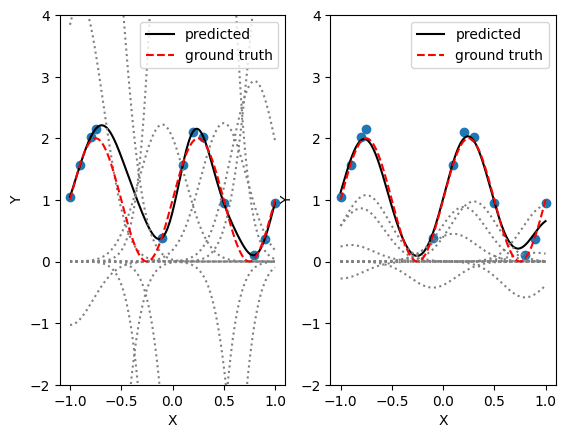
\includegraphics[width=0.7\textwidth]{Figures/ML-regularization.png}
    \caption{Zwei RBF-Modelle mit unterschiedlichen Regularisierungsparametern. 
    Links wurde der Regularisierungsparameter sehr klein gewählt. Entsprechend 
    sind die Basisfunktionen sehr gross und das Modell ist sehr komplex. Rechts
    wurde der Regularisierungsparameter grösser gewählt. Die Basisfunktionen sind
    kleiner und das Modell ist einfacher.}
    \label{fig:ml-regularisierung}    
\end{figure}

Eine ähnliche, aber noch mächtigere Möglichkeit, Eigenschaften von Lösungen zu definieren, bietet die 
\emph{Bayesianische Lineare Regression}. Hier nehmen wir an, dass die Parameter $w$ einer
Normalverteilung $w_i \sim N(0, \alpha)$ folgen. Auch dies hat den Effekt, das kleinere 
Parameterwerte bevorzugt werden. Im Gegensatz zu Ridge Regression erlaubt diese Formulierung 
eine komplett probabilistische Behandlung des Problems, und wir erhalten nicht nur den besten Parameterwert, sondern die Lösung ist  eine Wahrscheinlichkeitsverteilung $p(\textbf{w} | D)$ über gute Lösungen.
Abbildung~\ref{fig:ml-bayesian} zeigt	
ein Beispiel für eine Bayesianische lineare Regression. 
\begin{figure}[tb]
    \center
    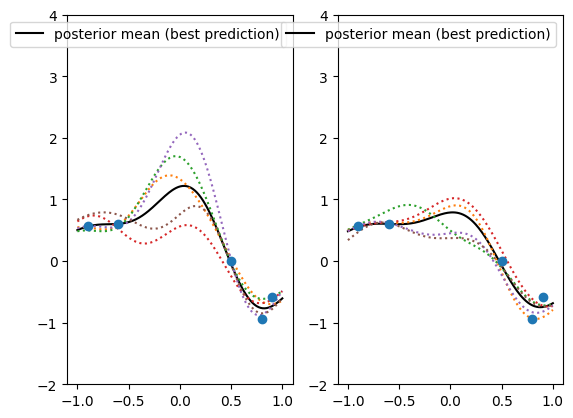
\includegraphics[width=0.7\textwidth]{Figures/ML-bayesian-regr.png}
    \caption{Ein Beispiel für eine Bayesianische Lineare Regression. Die schwarze Linie zeigt die 
    beste Vorhersage des Modells. Die gestrichtelten farbigen Linien zeigen zufällige 
    Stichproben der Posteriorverteilung $p(\textbf{w} | D)$. Beim Modell links 
    wurde die Varianz für den Prior auf die Gewichte gross gewählt. Deshalb 
    sind auch die möglichen Vorhersagen sehr unterschiedlich. Beim Modell rechts
    wurde die Varianz klein gewählt, und die möglichen Vorhersagen sind Entsprechend
    sehr viel enger verteilt.}
    \label{fig:ml-bayesian}    
\end{figure}

Sowohl Ridge regression als auch Bayesianische lineare Regression haben einfache 
analytische Lösungen, die ähnlich der Normalgleichungen durch
Linearen Gleichungssysteme gegeben sind. Die Details und ausführliche Diskussion dieser 
Methoden gehen aber über das Ziel dieser Vorlesung hinaus. 

.

\subsection{Neuronale Netze}

Wir haben gesehen, wie mir mit Basisfunktionsmodellen flexibel Modelle erstellen und damit auch nicht-lineare Zusammenhänge abbilden können. Durch die Wahl der Basisfunktionen 
sowie der Regularisierung können wir die Komplexität der Modelle steuern. 
Dank der linearen Struktur des Modells verfügen wir zudem eine einfache Möglichkeit,
die optimalen Gewichte zu bestimmen. 

Leider sind solche linearen Modelle für viele Anwendungen nicht flexibel genug. 
Wenn die Basisfunktionen nicht gut an die Charakteristiken der Daten angepasst sind, dann 
wird die Anzahl der Basisfunktionen, die
benötigt werden um komplexe Zusammenhänge zu modellieren, oft zu gross. Dies ist insbesondere dann der Fall, 
wenn die Daten hochdimensional sind.


Eine Möglichkeit, dieses Problem zu umgehen, ist die Verwendung von neuronalen Netzen.
Die Idee dahinter ist einfach: Statt im Voraus definierte Basisfunktionen zu verwenden, werden 
die Basisfunktionen selbst wieder parameterisiert, und die Parameter aus den Daten gelernt. 
Die Form der Basisfunktionen, die in diesem Kontext Neuronen, genannt werden, ist dabei wieder eine gewichtete 
Linearkombination aus den Eingaben.  Wir definieren  ein \emph{Neuron} $z(\textbf{x}, \textbf{w}$ mit Eingaben $\textbf{x} = (x_1, \ldots, x_m)$ und Parameter $\textbf{w} = (w_0, \ldots, w_1)$ wie folgt:
\[
   z(\textbf{x}, \textbf{w})=a(\sum_{i=1}^m w_{i}x_i + w_0).
\]
Damit auch nichtlineare Zusammenhänge repräsentiert werden können, wird auf das Resultat noch eine Aktivierungsfunktion $a$ angewendet. 
Einige Beispiele von Aktivierungsfunktionen sind in Tabelle \ref{ML:aktivierungsfunktionen} aufgeführt.

\begin{table}[h]
    \centering
    \begin{tabular}{lllll}
    \cline{1-2}
    \multicolumn{1}{|l|}{RELU}   & \multicolumn{1}{l|}{$a(x) = \mathrm{max}(0,x)$}              &  &  &  \\ \cline{1-2}
    \multicolumn{1}{|l|}{$\sigma$} & \multicolumn{1}{l|}{$a(x) = \frac{1}{1+e^{-x}}$}    &  &  &  \\ \cline{1-2}
    \multicolumn{1}{|l|}{TANH}   & \multicolumn{1}{l|}{$a(x) = \frac{2}{1+e^{-2x}}-1$} &  &  &  \\ \cline{1-2}
                                 &                                                   &  &  & 
    \end{tabular}
    \caption{Häufig verwendete Aktivierungsfunktionen.}
    \label{ML:aktivierungsfunktionen}
\end{table}

Abbildung \ref{fig:ml-neuron} illustriert den Aufbau eines Neurons grafisch. 
Wegen der nicht-linearen Aktivierungsfunktion können die optimalen Parameter eines neurons nicht mehr
analytisch über die Normalgleichung bestimmt werden. Stattdessen 
müssen wir die Gewichte des Modells iterativ über ein Verfahren
 wie das Gradientenabstiegsverfahren bestimmen. Dafür haben wir jetzt flexible Blöcke, 
 mit denen wir komplexere Lernverhalten modellieren können. Wir können diese Neuronen nämlich nun hierarchisch anordnen, um ein \emph{Multi-layer Neural Network} zu erhalten. Multi-layer Neural networks bestehen aus mehreren Schichten von Neuronen, wobei die Neuronen in jeder Schicht mit den neuronen in der Nachfolgeschichtverbunden sind. Ein solches Netzwerk ist in Abbildung \ref{fig:ml-multi-layer} dargestellt.
\begin{figure}[h!]

    \begin{subfigure}[h]{0.45\textwidth}
        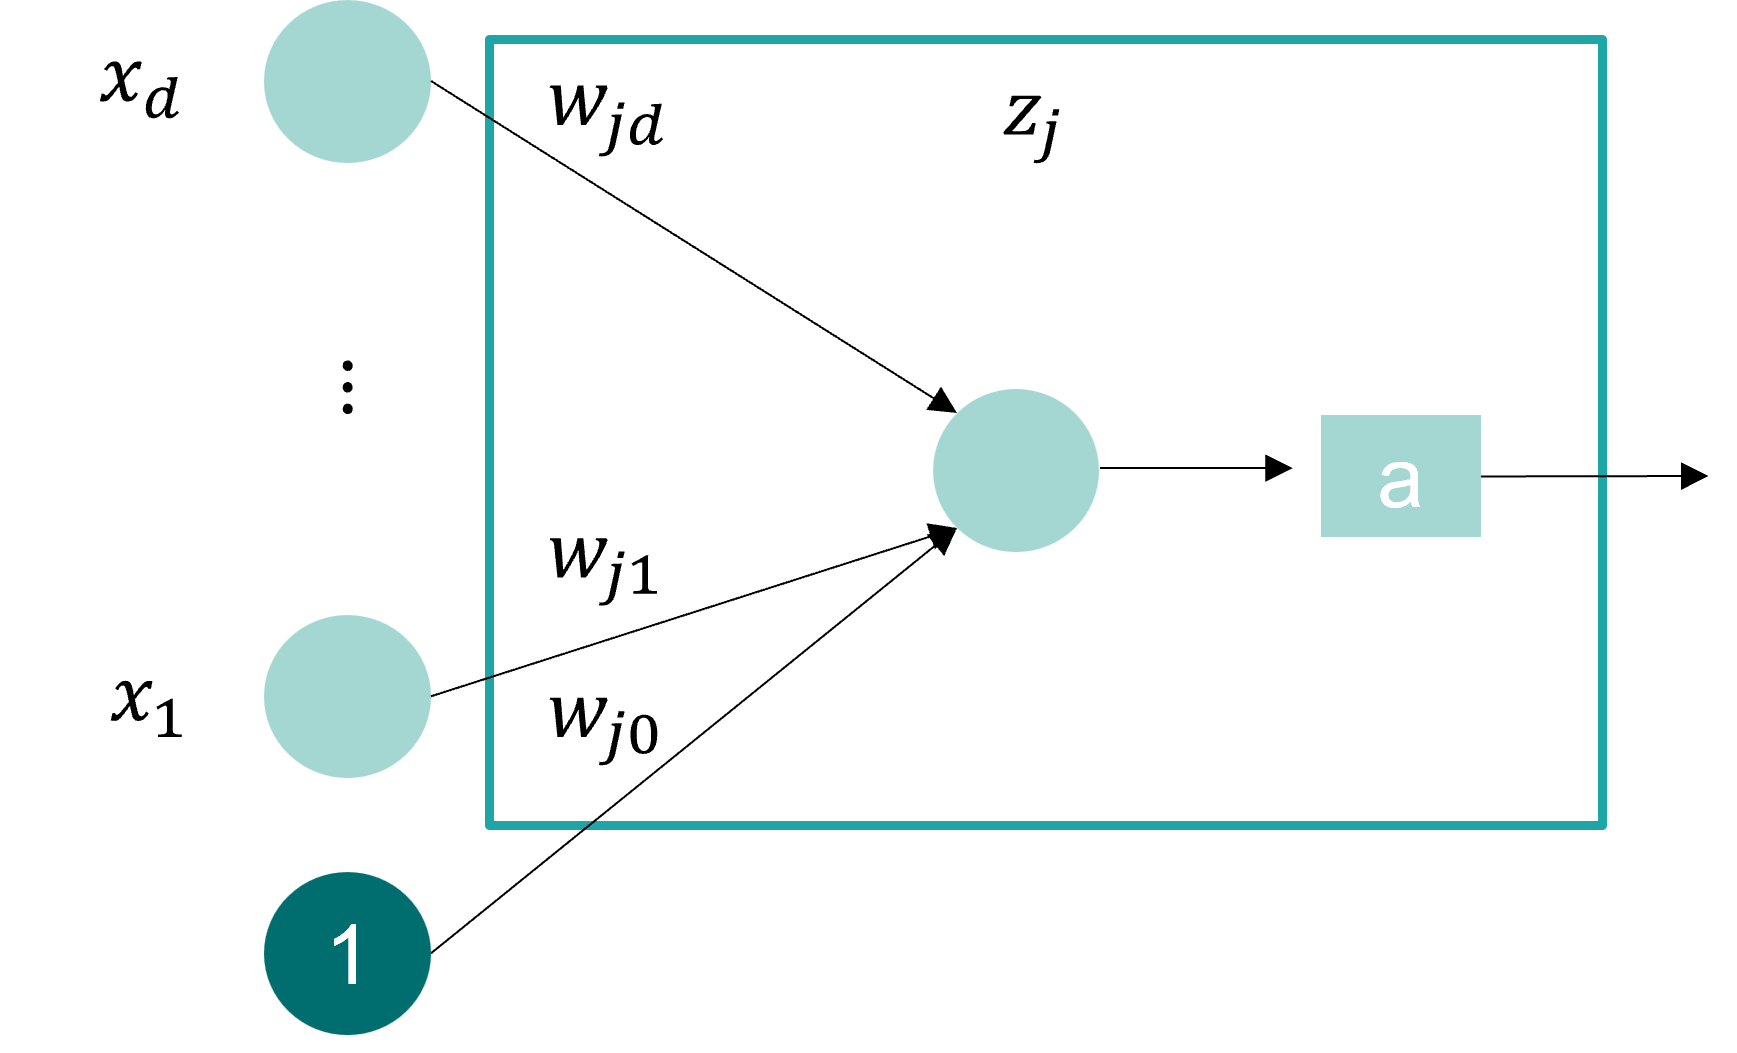
\includegraphics[width=\textwidth]{Figures/ML-neuron-2.png}
        \caption{}
        \label{fig:ml-neuron}
    \end{subfigure}
    \hfill
    \begin{subfigure}[h]{0.5\textwidth}
        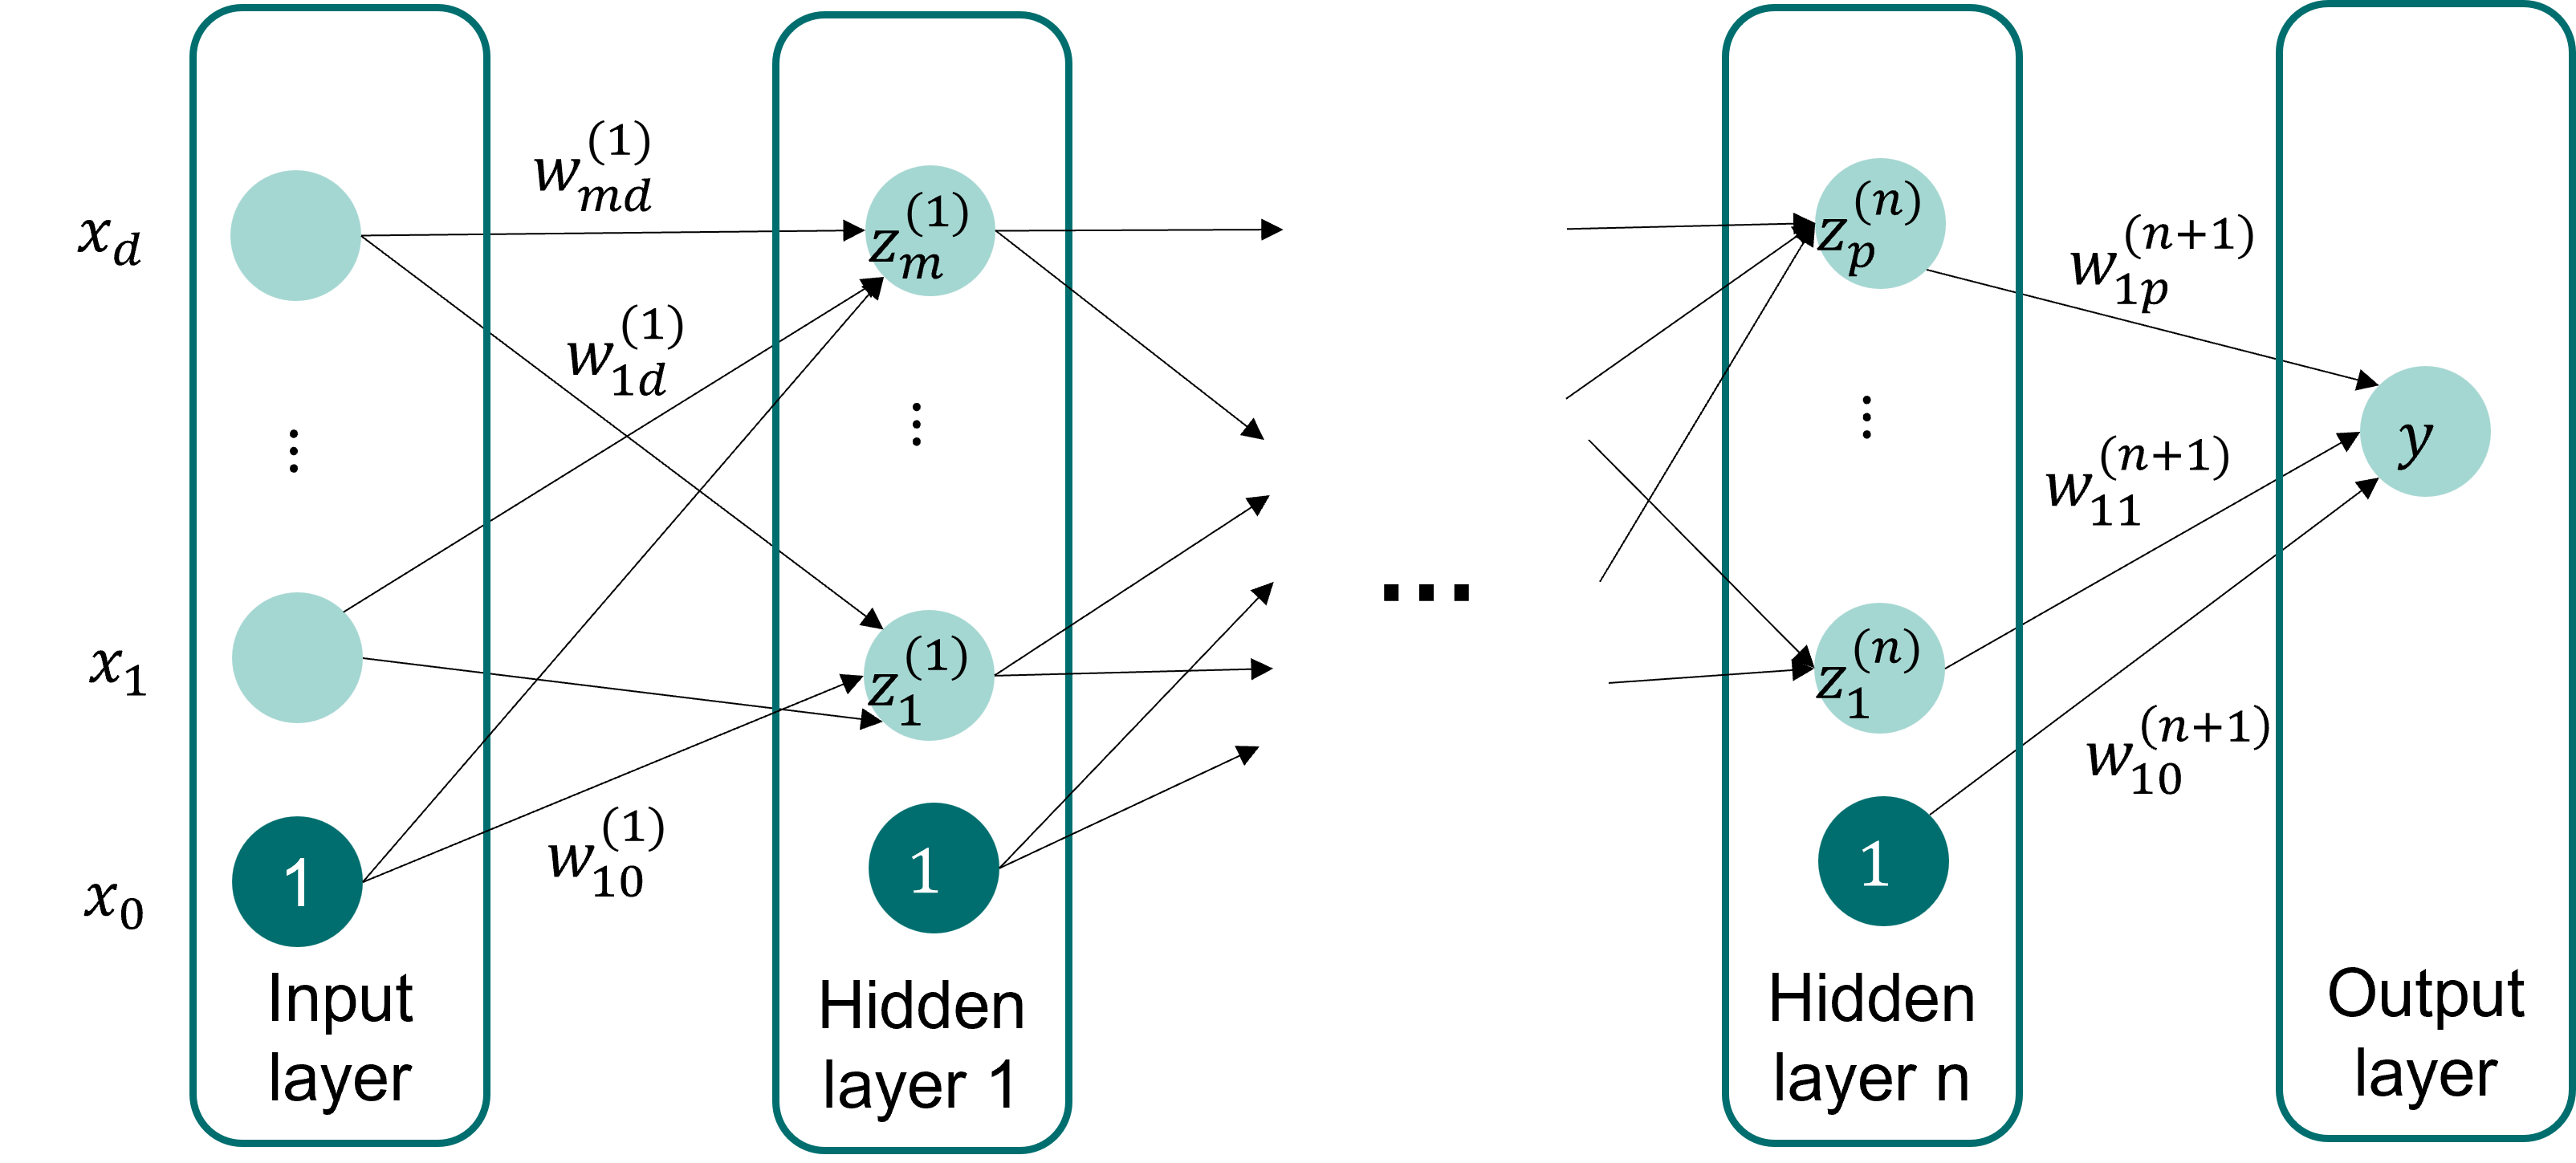
\includegraphics[width=\textwidth]{Figures/ML-multlayer-nn.png}
        \caption{}
        \label{fig:ml-basisfunktionen-mlp}
    \end{subfigure}
    \caption{\subref{fig:ml-neuron}) Schematische Darstellung eines Neurons. \subref{fig:ml-basisfunktionen-mlp}) Ein Neuronales Netz mit $n$ hidden Layer und einer einzigen Ausgabe $y$.}
    \label{fig:ml-multi-layer}        
\end{figure}

In unserer Interpretation von Neuronalen Netzen als Basisfunktionsmodelle, entsprechen die Neuronen in jeder Schicht den  Basisfunktionen, mit denen die Eingaben für die Neuronen in der nächsten Schicht transformiert werden. 
Die Eingaben, die die letzte Schicht erreichen sollten nach erfolgreichem Lernen so transformiert sein, 
dass eine einfache Linearkombination der Eingaben das in den Daten erhaltene Muster erklären kann. 

\subsubsection{Loss Funktionen für die Klassifizierung}

Wie oben besprochen benötigen wir für das Anpassen eines Modells an die Daten eine Verlustfunktion, welche die Differenz zwischen der Vorhersage des Modells $\hat{y} = f(x, \textbf{w})$ und dem
tatsächlichen Wert  $y$ misst. Für die Regression haben wir die quadratische Verlustfunktion $L(\hat{y}, y) = (f(x,\textbf{w}) - y)^2$ kennengelernt. Für Klassifizierungsprobleme, bei denen das Modell nur Vorhersagen muss, ob eine Eingabe $x$ 
zu einer bestimmten Klasse gehört, ist die Grösse des Abstands meist nicht von Interesse. Stattdessen wollen 
wir nur messen, ob wir die dem Label $y$ entsprechende Klasse gewählt haben. 

Wenn $y$ nur die Werte $0$ oder $1$ annehmen kann, verwenden wir dafür oft die \emph{Cross Entropy Loss Funktion}.
Die Cross Entropy Loss Funktion ist dann definiert als:
\[
    L(y, \hat{y}) = L(y, \sigma(f(x, \textbf{w}))) = -y \log(\sigma(f(x, \textbf{w}))) - (1-y)\log(1-\sigma(f(x, \textbf{w})))
\]
Dabei ist $\sigma(x)=\frac{1}{1+\exp(-x)}$ die Sigmoidfunktion, die den Wert von $f(x, \textbf{w})$ auf das 
Interval $[0,1]$ abbildet. Beachten Sie, dass der Verlust nur dann genau 0 wird wenn das Label mit der Vorhersage übereinstimmt. Ansonsten wird der Verlust positiv. 

%Wir können diese Funktion wieder durch einen Maximum Likelihood Schätzer motivieren.

% Dabei definieren wir die Likelihood Funktion als Bernoulliverteilung mit Parameter $\lambda$:
% \[
% p(y|\lambda) = (1-\lambda)^{1-y} \cdot \lambda^y      
% \]
% Der Parameter $\lambda$ soll dabei durch das Neuronale Netz bestimmt werden. 
% Da der Parameter $\lambda$ nur Werte zwischen 0 und 1 annehmen kann,
% verwenden wir als Aktivierungsfunkton im letzten Layer die Sigmoidfunktion $\sigma(x)=\frac{1}{1+\exp(-x)}$. 



%\section{Ausgewählte Modelle}\label{ml:modelle}
% \subsection{Entscheidungsbäume}
% Entscheidungsbäume sind eine einfache Art, Datensätze mit binären Merkmalen zu klassifizieren. Sie bestehen aus einer Wurzel, Knoten und Blättern. 
% Wurzeln und Knoten sind immer mit zwei Knoten oder Blättern verbunden und fragen immer nach einem bestimmten Merkmal in dem Datensatz. Abhängig von der Antwort wird man nach links oder nach rechts verwiesen. Die Konvention ist, dass eine ja-Antwort nach rechts und eine nein-Antwort nach links führt. Blätter sind die Enden vom Baum und geben  an, welches class label zu dieser spezifischen Kombination von Merkmalen gehört. Am besten stellt man sie grafisch dar ( z. B. Abb. \ref{fig:ml-baum}).\\

% \begin{figure}[h]
%     \centering
%     \includegraphics[scale=0.4]{Figures/ML-Baum.png}
%     \caption{Muster-Entscheidungsbaum aus der Vorlesung.}
%     \label{fig:ml-baum}
% \end{figure}

% Da Bäume theoretisch unendlich lang sein könnten, setzt man vorher eine Tiefe fest. Die Tiefe ist einfach die maximal erlaubte Anzahl von hintereinander gelegten Knoten. Wie man eine gute Tiefe wählen kann, werden wir später sehen.\\

% Eine praktische Verlustfunktion für Entscheidungsbäume ist:
% \begin{equation}
%     L(D,f) = \frac{\mathrm{Anzahl ~falsch ~klassifizierte ~Elemente ~in ~D}}{\mathrm{Anzahl ~Elemente ~in ~D}}~.
% \end{equation}
% \subsection{Lineare Regression}
% Lineare Regression verwenden wir, wenn sowohl die Merkmale als auch die class labels  Zahlen sind. 
% Für $n$ Merkmale ist unser Modell die Menge von allen $n$-dimensionalen Linearformen. 
% Die Vorhergesagte class label $y$ ist dann die Linearform angewendet auf die Merkmale.

% \begin{equation}
%     \mathcal{H} = \left\{ y=f(x_1,...,x_n) = \sum_{i=1}^n w_ix_i ~~|~w_1,..,w_n \in \mathbb{R}\right\}
% \end{equation}

% Die Verlustfunktion (auch \textit{Mean Squared Error} genannt) ist dann:
% \begin{equation}
%     L(D, f) = \mathrm{MSE}(D,f) = \frac{1}{m} \sum_{i=1}^m (f(x_{1,i},...,x_{n,i}) - y_i)^2
% \end{equation}
% wobei $m$ die Anzahl von Zeilen in $D$ und $(x_{1,i},...,x_{n,i},y_i)$ die Zeilen des Datensatzes sind.\\

% Um einzuschätzen, wie gut die Regression ist, bestimmen wir den \textbf{R2}-Wert eines Schätzers $f \in \mathcal{H}$. Wir definieren zuerst ein $f_0 = \frac{1}{n}\sum y_i$, der immer den Mittelwert der Trainingsdaten zurückgibt. Die R2-Score ist dann:
% \begin{equation}
%     R2(D,f) = 1 - \frac{\mathrm{MSE}(D,f)}{\mathrm{MSE}(D,f_0)}
% \end{equation}


% Ein negativer R2-Wert bedeutet, dass der Schätzer schlechter ist, als einfach immer den Mittelwert zurückzugeben. Je näher der R2-Wert an 1 ist, desto besser ist f. 

% \subsection{Logistische Regression}
% Logistische Regression wird verwendet, wenn man ein binäres class label und skalare Merkmale hat. Eine grafische Darstellung ist das Teilen des kartesischen Koordinatenraums in zwei Gebiete (siehe Abb. \ref{fig:ml-div}).

% \begin{figure}[h]
%     \centering
%     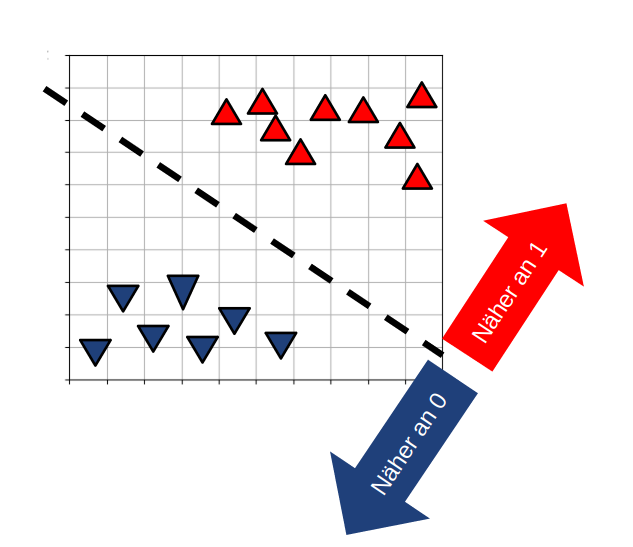
\includegraphics[scale=0.27]{Figures/ML-divided space.png}
%     \caption{Beispiel für logistische Regression aus der Vorlesung.}
%     \label{fig:ml-div}
% \end{figure}

% Dafür verwenden wir das Modell:
% \begin{equation}
%         \mathcal{H} = \left\{ y=f(x_1,...,x_n) = \sigma (w_0 + w_1*x_1 + ... + w_n*x_n) ~~|~w_0,..,w_n \in \mathbb{R}\right\}
% \end{equation}
% wobei  $\sigma$ die Sigmoidfunktion $\sigma: \mathbb{R} \to (0,1)$ ist. \footnote{Die Verlustfunktionen sind mathematische Normen für den Funktionenraum $L^2$ (nicht klasurrelevant, für mehr Information MMP I)}

\section{Training von Machine Learning Modellen}
Mit linearen Basisfunktionen und neuronalen Netzen haben wir nun zwei Modelle kennengelernt, die uns erlauben, komplexe Zusammenhänge in den Daten zu modellieren. Wir haben aber auch schon gesehen, dass komplexe Modelle dazu neigen, die Daten zu \emph{überfitten}. Das bedeutet, dass das Modell die Daten nicht nur gut erklärt, sondern auch das Rauschen in den Daten ``lernt''. Das kann die Nützlichkeit des Modells für Voraussagen stark einschränken.

In der Praxis müssen wir sicherstellen, dass unser Modell nicht nur die Trainingsdaten
gut erklärt, sondern auch auf neuen Daten gut funktioniert.
Um dies zu erreichen, verwenden wir oft eine \emph{Trainings-Validierungs-Test} Aufteilung.
Die Trainingsdaten werden verwendet, um das Modell zu trainieren. Die Validierungsdaten
werden verwendet, um die Hyperparameter des Modells zu optimieren. Die Testdaten werden
verwendet, um die Performance des Modells zu evaluieren.

\subsection{Hyperparameteroptimierung}
Die Wahl der Hyperparameter ist ein wichtiger Schritt im Machine Learning.
Hyperparameter sind Parameter, die nicht durch das Modell gelernt werden, sondern
vor dem Training festgelegt werden müssen. Beispiele für Hyperparameter sind die
Anzahl der Basisfunktionen in einem Basisfunktionsmodell, die Breite einer Radialen 
Basisfunktion oder die Anzahl der Schichten und Neuronen in einem neuronalen Netz.

Die Wahl der Hyperparameter ist oft nicht trivial und kann einen grossen Einfluss auf die
Performance des Modells haben. Eine Möglichkeit, die Hyperparameter zu optimieren, ist
die \emph{Grid Search}. Dabei wird ein Gitter von Hyperparametern definiert, und für
jede Kombination von Hyperparametern wird das Modell trainiert und auf den Validierungsdaten
evaluiert. Die Hyperparameter, die die beste Performance auf den Validierungsdaten liefern,
werden dann für das finale Modell verwendet.

\subsection{Crossvalidation} \label{ML-Crossval}
Eine weitere Möglichkeit, die Performance des Modells zu evaluieren, ist die \emph{Crossvalidation}.
Dabei wird der Datensatz in $k$ Teile aufgeteilt. Das Modell wird dann $k$ mal trainiert und
evaluiert, wobei jedes Mal ein anderer Teil des Datensatzes als Validierungsdaten verwendet wird.
Die Performance des Modells wird dann als Durchschnitt der Performances über alle $k$ Durchläufe
berechnet.

% Sei $D$ der Datensatz, $\mathcal{H}_n$ Entscheidungsbäume der Tiefe $n$, und $f_{n,D^*} \in \mathcal{H}_n$ der Baum, der eine Verlustfunktion auf $D^*$ minimiert. Mit den folgenden Methoden kann man eine gute Tiefe finden.
% \subsection{Crossvalidation} \label{ML-Crossval}
% \begin{enumerate}
%     \item Teile D in ein \textit{training} Dataset $D^*$ und ein \textit{validation} Dataset $D'$. Oft ist das Training-Dataset länger. 
%     \item Wähle Tiefen $t_1,...t_i$, die untersucht werden sollen.
%     \item Finde $f_{t_1,D^*},...,f_{t_i,D^*}$ durch das Training und berechne $L(D',f_{t_1,D^*}),...,L(D',f_{t_i,D^*})$
%     \item  Die Tiefe mit dem minimalen Verlustwert in 3. ist die optimale Tiefe.

% \end{enumerate}
% \subsection{k-Fold Crossvalidation}
% \begin{enumerate}
%     \item Teile $D$ in $k$ gleichlange Teile. Wir nennen diese $D_1,...,D_k$. 
%     \item Für jedes $D_i$ führe crossvalidation \ref{ML-Crossval} mit $D_i$ als \textit{validation} Dataset und Rest von D als \textit{training} Dataset aus. 
%     \item Die Tiefe, die am häufigsten den minimalen Verlustwert hatte, ist die optimale Tiefe. 
% \end{enumerate}

\section{Deep Learning}

Die zurzeit unbestritten populärste Form von Machine Learning ist \textit{Deep Learning}. 
Deep Learning ist eine spezielle Form von Machine Learning, die auf neuronalen Netzen basiert.
Der Begriff deep learning kommt daher, dass die neuronalen Netze oft sehr tief sind, d.h. viele Schichten haben.
Es gibt natürlich zahlreiche Möglichkeiten, ein neuronales Netz zu konstruieren. Je nach Anwendung kommen 
verschiedene Architekturen zum Einsatz. In diesem Abschnitt werden wir einige der wichtigsten Architekturen vorstellen.

\subsection{Convolutional Neural Networks}
Das Hauptziel von CNNs ist Bilderkennung. Wir möchten immer noch Objekte voneinander unterscheiden, aber statt skalarer Merkmale möchten wir jetzt Bilder betrachten. Als erste Idee könnten wir jeden Pixel als Eingang zu einem neuronalen Netz nehmen und ein riesiges Netzwerk verwenden, um die Klassifikation durchzuführen. Aber dafür bräuchten wir zu viele Neuronen. Stattdessen verwenden wir \textit{convolution} \footnote{Convolution ist hier nicht im Sinne von \textit{Complex} (convoluted), sondern im Sinne von \textit{Faltung} zu verstehen. }, um die Bilder zu vereinfachen. Für Faltung betrachten wir Bilder als Matrizen. Sei $E \in \mathbb{R}^{nxn}$ die zu faltende Matrix und $F \in {0,1}^{2x2}$ die Faltungsmatrix. Der Ausgang ist $A \in \mathbb{R}^{n-1xn-1}$. \footnote{Falls $n$ kein ganzzahliges Mehrfaches von der Größe von $F$ ist, dann vernachlässigt man genügend der letzten Zeilen und Spalten von $E$.}
\begin{equation}
    A_{i,j} = E_{i,j}F_{1,1} + E_{i+1,j}F_{2,1} + E_{i,j+1}F_{1,2} +E_{i+1,j+1}F_{2,2}     
\end{equation}
Man stellt dies am besten grafisch dar: Man legt die Faltungsmatrix auf jeden 2x2 Block in $E$, multipliziert die Einträge, die aufeinander liegen, summiert die Ergebnisse, und notiert die Summe auf einer neuen Matrix für jeden 2x2 Block in $E$. \\

Man kann noch einen Filter (Aktivierungsfunktion) auf das Ergebnisse anwenden. Zum Beispiel:
\begin{equation}
        A_{i,j} = RELU( E_{i,j}F_{1,1} + E_{i+1,j}F_{2,1} + E_{i,j+1}F_{1,2} +E_{i+1,j+1}F_{2,2} )
\end{equation}

Eine weitere Methode, die für CNN verwendet wird, ist \textit{Pooling}. Es wird ähnlich wie Faltung angewendet, aber es keine lineare Funktion, sondern \textit{max} oder \textit{min}:
\begin{equation}
    A_{i,j} = \mathrm{max}\{E_{i,j};E_{i+1,j};E_{i,j+1};E_{i+1,j+1}\}
\end{equation}

Eine geschickte Wahl von Faltungsschichten führt nicht nur zu einer Reduktion der Bilddimension, sondern auch zu Hervorhebung von Merkmalen (Kanten, Ecken etc.) des gesuchten Objekts (siehe Abb. \ref{fig:ml-conv}. Man kann die "gefalteten" Bilder dann mithilfe eines neuronalen Netzes klassifizieren.

\begin{figure}[h]
    \centering
    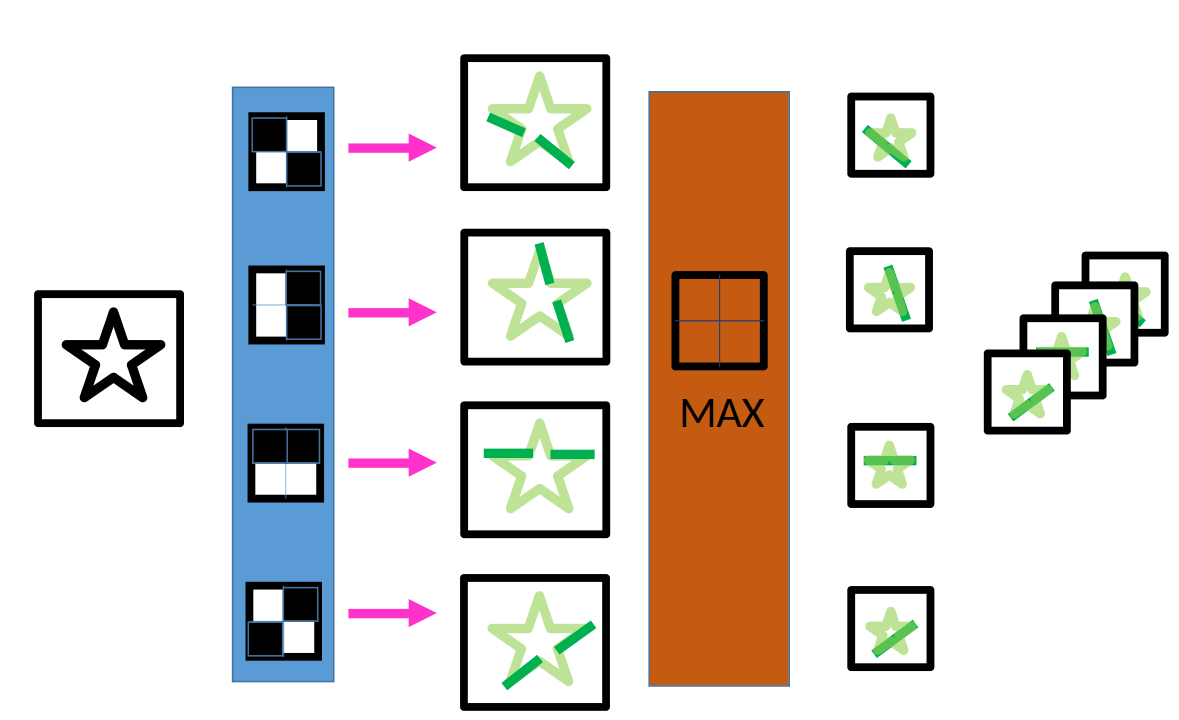
\includegraphics[scale= 0.3]{Figures/ML-conv.png}
    \caption{Hier werden die Kanten von einem Stern mit einem CNN hervorgehoben. Die nachfolgenden neuronalen Netze können dann aus den Kanten entscheiden, ob es einen Stern ist.}
    \label{fig:ml-conv}
\end{figure}
\subsection{Andere Architekturen}
\subsubsection{Autoencoder}
Ein Autoencoder besteht aus einem Encoder und einem Decoder. Der Encoder überführt die Eingangsinformation (Bild oder Data) in einen mehrdimensionalen Raum (auch Code Space genannt). Der Decoder ist die umgekehrte Operation. Die Idee ist, dass ähnliche Eingänge näher zu einander im Code Space abgebildet werden. Dann können wir mithilfe von Clustering die Daten klassifizieren. Ein Beispiel ist Schrifterkennung. Bilder von Schriftzeichen werden mithilfe von einem Encoder auf dem Code Space abgebildet. Dann können wir aus der Position im Code Space erkennen, welches Schriftzeichen es war.\\

Der Encoder und Decoder sind neuronale Netze, die auch trainiert werden müssen. Die Layer sind Sanduhr artig, dies führt dazu, dass nur die wichtigste Information im Code Space abgebildet wird. Was diese Information (bzw. was die Achsen von Code Space) bedeuten ist a priori unbekannt. Die Verlustfunktion für Training ist:
\begin{equation}
    L(D, Enc,Dec) = \sum_{x\in D} || x -Dec(Enc(x))||^2
\end{equation}

\subsection{Generative Adversarial Networks (GAN)}
GANs sind dafür geeignet, um Bilder zu generieren oder zu verändern. Ein GAN hat einen Generator, der Bilder generieren kann und einen Diskriminator, der Bilder beurteilen kann. Der Diskriminator versucht die Bilder vom Generator von echten Bildern unterscheiden zu können. Der Generator versucht Bilder, die vom Diskriminator als ``echt`` gesehen werden, zu generieren.

\section{Kodierung kategorischer Daten}
Wie wir gesehen haben, arbeiten alle bisherige Modelle auf numerischen Daten (entweder {0,1} oder $\mathbb{R}$), aber im reellen Leben sind Daten oft nicht numerisch, sondern kategorisch \footnote{z.B Gender wird oft mit männlich, weiblich oder divers bezeichnet. Diese lassen sich aber nicht natürlicherweise mit Zahlen ausdrücken. }. Deshalb müssen wir uns bewusst eine Codierung auswählen. In dem folgenden Paragrafen betrachten wir verschiedene Methoden anhand des Titanik-Dataset (siehe Abbildung \ref{fig:titanik-dataset}).

\begin{figure}
    \centering
    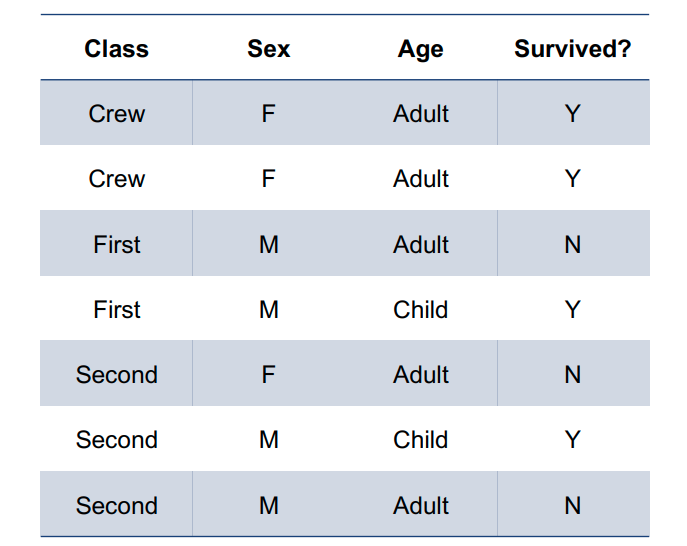
\includegraphics[scale=0.4]{Figures/Ml-Titanik-Dataset.png}
    \caption{Auszug des Titanik Datasets. }
    \label{fig:titanik-dataset}
\end{figure}
\subsection{Ordinal Encoding}
Dies ist die einfachste Methode. Mögliche Kategorien jedes Merkmals werden mit arbiträren ganzen Zahlen bezeichnet. Zum Beispiel im Titanik-Dataset können wir für das Merkmal \textit{class} Crew mit 1, First mit 2 und Second mit 3 bezeichnen. Obwohl wir die Zahlen willkürlich gewählt haben, haben wir plötzlich Crew näher mit First als mit Second platziert. Das kann  in der Auswertung nachteilig sein.

\subsection{Mean Encoding}
Hier bezeichnen wir jede Kategorie mit einem Mean, der mit Hilfe von dem \textit{class label} generiert wird. In unserem Fall können wir dieses Mean als Überlebenschance nehmen. Für \textit{Age} Merkmal bezeichnen wir \textit{Kind} mit 1, denn jedes Kind hat überlebt, und \textit{Adult} mit 0.4, denn 40 \% der Erwachsene haben überlebt. Nachteil ist, dass wir plötzlich Information aus dem \textit{class label} in die Merkmale übertragen haben. Dies kann zu Overfitting führen.

\subsection{One-Hot Encoding}
Für diese Methode machen wir aus einem Merkmal mit $n$ Kategorien $n$ Merkmale, d.h. z. B. für das Merkmal \textit{class}: Es gibt jetzt drei Merkmale mit Werten {0,1}. Diese sind ''Ist Crew?'', ''Ist First?'' und ''Ist Second?''. Dadurch haben wir keinen der Nachteile der vorherigen Methoden, aber unser Datensatz ist \textit{viel}\footnote{Der Titanik-Datensatz hat nach One-Hot Encoding ca. 2 mal mehr Merkmale.} größer geworden. 


\section{Clustering \& K-Means-Methode}
Wir möchten unsere Daten mit skalaren Merkmalen (z.B. Helligkeit und Größe für Sterne) gemäß ihrer Entfernung zueinander in Clusters (Bündel) sammeln. Die k-Means-Methode dient dazu, die geeigneten Bündel zu finden. Unser Modell ist
\begin{equation}
     \mathcal{H} = \left\{ (\theta_1,...,\theta_k,c) | \theta_1,...,\theta_k \in \mathbb{R}^d \land c : \mathbb{R}^d \to \{1,...,k\} \right\}
\end{equation}
wobei wir k Bündel mit Mittelpunkt (auch Zentroid benannt) $\theta$ und die Zuweisungsfunktion $c$ betrachten. Die Funktion $c$ gibt für jeden Punkt in $\mathbb{R}^d$ an, zu welchem Bündel dieser Punkt gehört. Zu bemerken ist, dass dies kein neuronales Netz ist. Die Verlustfunktion ist so gedacht, dass der Abstand der Punkten zu ihrem zugewiesenen Cluster-Mittelpunkt bestraft wird. Wir formalisieren dies wie folgt:\\

$D \subseteq \mathbb{R}^d$ sind die gegebenen Punkte,  $\{\theta_1,...,\theta_k\} \subseteq \mathbb{R}^d$ die Cluster-Mittelpunkte, $c$ die Zuwesiungsfunktionen. Dann ist die Verlustfunktion: 
\begin{equation}
    \mathcal{L}(D,\theta_1,...,\theta_k,c) = \sum_{x \in D} || x - \theta_{c(x)}||^2 
\end{equation}
Bemerkung: $\theta_{c(x)}$ ist der  $x$ zugewiesene Mittelpunkt.\\

Für das Training verwenden den folgenden Algorithmus:

\begin{itemize}
    \item \textbf{Gegeben: } $D \in \mathbb{R}^d$
    \item \textbf{Initialisierung: } wähle $\theta_1,...,\theta_k$ zufällig. 
    \item \textbf{Zuweisung aktualisieren: } wir setzen $c(x) = argmin_{j \leq k} || x -\theta_j||$. Dies bedeutet, dass jedem Punkt der nächstgelegene Cluster-Mittelpunkt zugewiesen wird.
    \item \textbf{Cluster-Mittelpunkte aktualisieren: } Sei $S_j = \left\{ x \in D | c(x) = j\right\}$ die Menge der Punkte in Cluster $j$. $\forall j \leq k$ setze $\theta_j = \frac{1}{|S_j|} \sum_{x \in S_j} x$. Somit haben wir alle Cluster-Mittelpunkte auf den wirklichen Mittelpunkt des Clusters gesetzt.
    \item Führe die Aktualisierung-Schritte immer wieder durch, bis die Clusters sich nicht mehr ändern. 
\end{itemize}
\begin{figure}
    \centering
    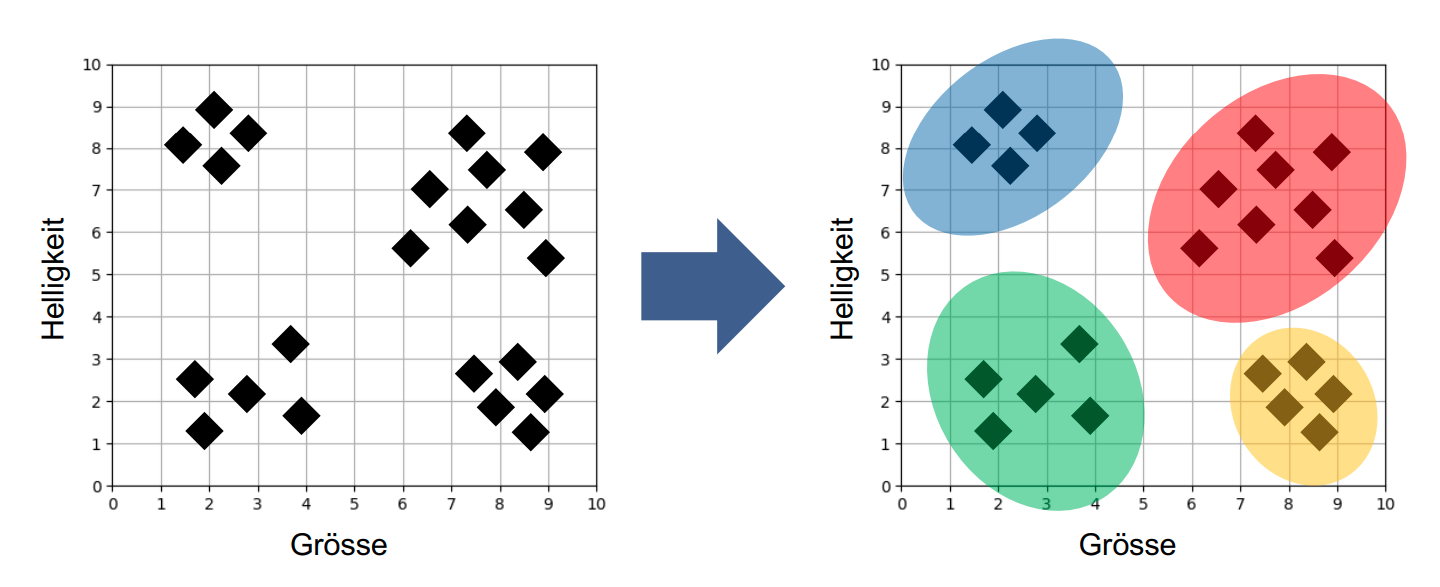
\includegraphics[scale=0.3]{Figures/ML-Clustering.png}
    \caption{Graphische Vorstellung des Clustering.}
\end{figure}
\subsection{Overfitting}
Wenn wir $k$ zu gross wählen (z.B  $k \geq |D|$), dann ist die beste Zuordnung immer einen Punkt pro Cluster. Wir können dies  nicht mit Cross-Validation (siehe \ref{ML-Crossval}) bemerken, denn $\mathcal{L}$ strebt gegen 0 für $k$ gegen $|D|$. Wenn wir mit Cross-Validation Overfitting verhindern wollen, dann müssen wir die Verlustfunktion so verändern, sodass sie auch große k bestraft. Wir verwenden mit $\lambda > 0$:
\begin{equation}
    L = \mathcal{L} + \lambda e^k
\end{equation}
Jetzt können wir Cross-Validation verwenden, um die optimale Anzahl Clusters zu finden. 

\section{Principal Component Analysis (PCA)}
Als Letztes betrachten wir die PCA, was dafür gedacht ist, die Dimension (Anzahl Merkmale) ohne große Verluste von Information zu reduzieren. Dies ist nützlich, weil so unsere anderen Modelle schneller und korrekter funktionieren, wobei besonders wichtig ist, dass sie korrekter werden. Mit einer hohen Anzahl von Merkmalen wird der Suchraum $\mathbb{H}$ größer und es kann sein, dass wir nicht die perfekte Lösung finden.

Formell ist PCA eine Methode unseren Datensatz $\{x_1,...,x_n\} \subseteq \mathbb{R}^D$\footnote{Die $x_i$'s sind die Zeilen des Datensatzes und  $D$ ist die Anzahl von Merkmalen. } auf einem reduzierten Datensatz $\{t_1,...,t_n\} \subseteq \mathbb{R}^d$ abzubilden. Aus Lineare Algebra Perspektive ist die PCA eine Abbildung auf einen Unterraum. Wir möchten allerdings  so viel Information wie möglich behalten. Die Abbildung wird $\forall i \leq n$ folgenderweise definiert:
\begin{equation}
    t_i = (x_i \cdot w_1 ,... x_i \cdot w_d)^T
\end{equation}
wobei $\{w_1,...,w_d\} \subseteq \mathbb{R}^D$ die Gewichtsvektoren sind. 

\textbf{\textit{Fall 1: d=1}}\\


In diesem Fall suchen wir nur die $w_1$, sodass $t_i = (x_i \cdot w_1) \in \mathbb{R}$ die  Streuung  $\sum t_i^2$ maximiert. Sei \textbf{X} die $n\times D$ Matrix, die in jeder Zeile ein Element aus dem Datensatz hat.

\begin{equation}
    X = \begin{pmatrix}
        - ~x_1~ -\\
        - ~ x_2 ~ - \\
        .\\.\\.\\
        -~x_n~-
        \end{pmatrix}\\
\end{equation}
Dann können wir $w_1$ mit Hilfe folgender Gleichung finden: 
\begin{equation}
    w_1 = argmax_{||w|| = 1}\left\{ \sum_i^n (x_i\cdot w_n)^2 \right\}= argmax_{||w|| = 1} \left\{||\textbf{X}w||^2\right\}
\end{equation}
Die Ausdruck $||\textbf{X}w||^2$ wird maximal, wenn $w$ der Eigenvektor $u_1^*$ zum größten Eigenwert $\lambda_1^*$ ist. Dies kann mit Methoden aus der linearen Algebra finden. \\

\textbf{\textit{Fall 2: $d \geq 1$}}\\

In diesem Fall suchen wir $d$ Gewichtsvektoren. $w_1$ ist wieder wie in Fall 1 zu finden, für die $w_2$ subtrahieren wir die Projektion von $x$ auf den Unterraum \textit{Spann}{$[w_1]$} von $x$ für jedes $x \in X $ also:
\begin{equation}
    X_1 = \{x - proj_{u_1}^* x | x \in x\} = \{x - (x \cdot u_1^*)u_1^* | x \in x\}
    \label{eq_ml_proj_set}
\end{equation}
Dann können wir noch einmal die Methode von Fall 1 (aber jetzt mit $X_2$ als Datensatz) anwenden, um $w_2$ zu bestimmen. Folglich können wir mit mehrmaligem Anwenden $(w_1,...,w_d)$ bestimmen. Formell geschrieben:

\begin{align}
    \textbf{X}_k &= \textbf{X} - \sum_{s=1}^{k-1} \textbf{X}w_s w_s^T\\ \label{eq_ml_mat_proj}
    w_k &=  argmax_{||w|| = 1} \left\{||\textbf{X}_k w||^2\right\}
\end{align}
Die Gleichung \ref{eq_ml_mat_proj} ist äquivalent zu mehrmaligen Anwenden von Gleichung \ref{eq_ml_proj_set}.
